\section{Resultater \& diskussion}

    \subsection{Smeltepunkt og TLC}
    \begin{figure}[H]\centering
        \caption{Smeltepunkt og RF (retentionsfaktor) for stof dannet ved de 3 synteser, samt sammenligning med teoretiske værdier for kommercielt stof.}
        \begin{tabular*}{\linewidth}{c@{\extracolsep{\fill}}cccccccc}
            \toprule
            & & & & & \multicolumn{4}{c}{Syntese 3} \\
            \cmidrule(r){6-9}
            & \multicolumn{2}{c}{Syntese 1} & \multicolumn{2}{c}{Syntese 2} & \multicolumn{2}{c}{Ethyl} & \multicolumn{2}{c}{Propyl} \\
            \cmidrule(r){2-3} \cmidrule(r){4-5} \cmidrule(r){6-7} \cmidrule(r){8-9}
            Prøve \# & SMP & RF & SMP & RF & SMP & RF & SMP & RF \\
            \midrule
            1 & 116 & 0.24 & 95 & 0.63 & 116 & 0.50 & 96 & 0.49 \\
            2 & 115 & 0.20 & 96 & 0.67 & 116 & 0.49 & 93 & 0.45 \\
            3 & 116 & 0.21 & 96 & 0.59 & 117 & 0.49 & 94 & 0.45 \\
            \midrule
            Teoretisk & 117 & 0.22 & 97 & 0.63 & 117 & 0.49 & 97 & 0.46 \\
            Gennemsnit & 116 & 0.22 & 95.7 & 0.63 & 116.3 & 0.49 & 94.3 & 0.46 \\
            \midrule
            Afvigelse $\left[\si{\%}\right]$ & -1 & 0 & -1 & 2 & -1 & 0 & -3 & 0 \\
            \bottomrule
        \end{tabular*}
    \end{figure} \vskip -8pt
    Med udgangspunkt i hhv.\ smeltepunkts-- samt TLC--analysen vil det være rimeligt at antage at det dannede stof sandsynligvis er hvad vi tror det er. De relativt høje afvigelser for smeltepunktet hos propylparaben kan hovedsageligt tilskrives større partikelstørrelse, da pulveret var svært at knuse ordentligt hvilket medførte mindre tæt pakning.

    \subsection{H--NMR--spektroskopi}
    Vi undersøger først spektret for ethylparaben og vurderer om det er sandsynligt at det dannede H NMR-spektrum passer til det vi ville forvente. Til dette formål kigger vi på de individuelle peaks da antallet af spidser kan give os en ide om hvilke atomer de korresponderer til.
    \begin{figure}[H] \centering
        \includegraphics[width=\textwidth,page=2]{bilag/ethylnmr}
        \caption{Peaks for H--NMR analyse af ethylparaben.}
    \end{figure} 
    Peaket omkring $\delta=1.28\si{ppm}$ forventes at være tilsvarende methylgruppen på forgreningen der udgår fra benzenringen, eftersom vi observerer 3 peaks, må atomet hydrogenerne er bundet til have 2 naboprotoner, hvilket kun opfyldes af methylengruppen. Ved $\delta=4.25\si{ppm}$ ses 4 peaks, altså må det være methylengruppen idet den har 3 naboprotoner fra methylgruppen. 
    
    Omkring $\delta=6.84\si{ppm}$ forventer vi hydrogenerne bundet til carbonatomerne i meta-positionerne i benzenringen, idet de vil have et lavere kemisk skift end dem i ortho-positionen grundet den øgede elektronegativitet fra oxygenatomet der er til stede i phenolgruppen. 
    
    I selve spektret ses også en singlet ved $\delta=10.25\si{ppm}$, dette kemiske skift er højere end hvad vi normalt villet forvente for en phenolgruppe (der normalt villet befinde sig omkring det aromatiske område, ligesom ortho- og meta-carbonatomerne). Dette kan begrundes i det benyttede opløsningsmiddel, DMSO-d6, da det har mulighed for at danne hydrogenbindinger med phenolgruppen \parencite{Raym2007}
    \begin{figure}[H]\centering
        \resizebox{\textwidth}{!}{
        \schemestart
        \chemfig{HO-*6(=-=(-COOR)-=-)}
        \+
        \chemfig[-32pt]{S(-[7]CD3)(-[5]CD3)(=[2]O)}
        \arrow(.mid east--.mid west){->}
        \chemfig{O(=[5]S(-[3]CD3)(-[6]CD3))-[2,,,,thick,dotted,red]H(-[1]O-*6(=-=(-COOR)-=-))}
        \schemestop
        }
        \caption{Dannelse af hydrogenbinding mellem DMSO-d6 og vilkårlig paraben.}
    \end{figure}
    Dette medfører at deres elektronegativitet ``mødes i midten'', hvorved den lokale elektrondensitet på hydrogenatomet (og derved beskyttelsen mod $B_0$) øges drastisk.
    \begin{figure}[H] \centering
        \includegraphics[width=\textwidth,page=2]{bilag/propylnmr}
        \caption{Peaks for H--NMR analyse af propylparaben.}
    \end{figure} 

    \subsection{IR--spektroskopi}


    \subsection{Hæmningsforsøg}
    

